\documentclass[11pt,a4paper]{article}
\usepackage[utf8]{inputenc}
\usepackage[T1]{fontenc}
\usepackage[francais]{babel}
\usepackage{amsmath}
\usepackage{amsfonts}
\usepackage{amssymb}
\usepackage{graphicx}
\usepackage{fullpage}
\usepackage{tikz}

\title{Sémantique TD2}

\begin{document}
	\section{Probabilité de mutation d'une lettre}
	\subsection{Énoncé}
	Trouver la probabilité qu'une lettre $B$ ne mute pas en une lettre $B^{\prime}$, en fonction du temps $t$.
	
	Avec :
	\begin{itemize}
		\item $P(t)$ la probabilité qu'une lettre B ne mute pas au temps $t$
		\item $\alpha_{T}$ la probabilité qu'une lettre B mute au temps $t$
		\item $B \in A = \{A, C, G, T\}$
		\item $B^{\prime} \in A, B^{\prime} \neq B$
	\end{itemize}
	\begin{align*}
		P(0) &= 1\\
		P(1) &=(1 - (n - 1)\alpha_{T}) P(0)\\
		P(2) &=(1 - (n - 1)\alpha_{T}) P(1) + \alpha_{T}(1 - P(1))\\
	\end{align*}
	
	\subsection{Explication}
	\begin{center}
	\begin{tikzpicture}[yscale=-1]
		\draw [->] (3,0) -- (3,4);
		\draw (3,0) node[right] {$t_{0}$};
		\draw (3,2) node[right] {$t_{1}$};
		\draw (3,4) node[right] {$t_{2}$};
		\node[shape=circle,draw=black] (0) at (0,0) {$B$};
		\node[shape=circle,draw=black] (1) at (-1,2) {$B$};
		\node[shape=circle,draw=black] (2) at (1,2) {$B^{\prime}$};
		\node[shape=circle,draw=black] (3) at (0,4) {$B$};
		\path [->] (0) edge node[left] {$1-(n-1)\alpha_{T}$} (1);
		\path [->] (0) edge node[right] {$\alpha_{T}$} (2);
		\path [->] (1) edge node[left] {$1-(n-1)\alpha_{T}$} (3);
		\path [->] (2) edge node[right] {$\alpha_{T}$} (3);
	\end{tikzpicture}
	\end{center}

	\subsection{Formule générale}
	
	Déterminer la relation de récurrence $P(t + T)$ vérifiée pour tout $t$ :\\
	$$P(t + T) = (1 - (n - 1)\alpha_{T})P(t) + \alpha_{T}(1 - P(t))$$
	Déterminer la formulation générale de la relation de récurrence $P_{B}(t + T)$ vérifiée pour tout $t$ et en introduisant $P_{B}(t), P_{B^{\prime}}(t), P_{T}(B \to B^{\prime})$ et plusieurs taux de substitution $P_{T}(B \to B^{\prime})$
	
	\newpage
	
	\section{Le moment ou tout part en couilles}
	
	Il a effacé <3\\
	
	\begin{figure}[ht]
		\centering
		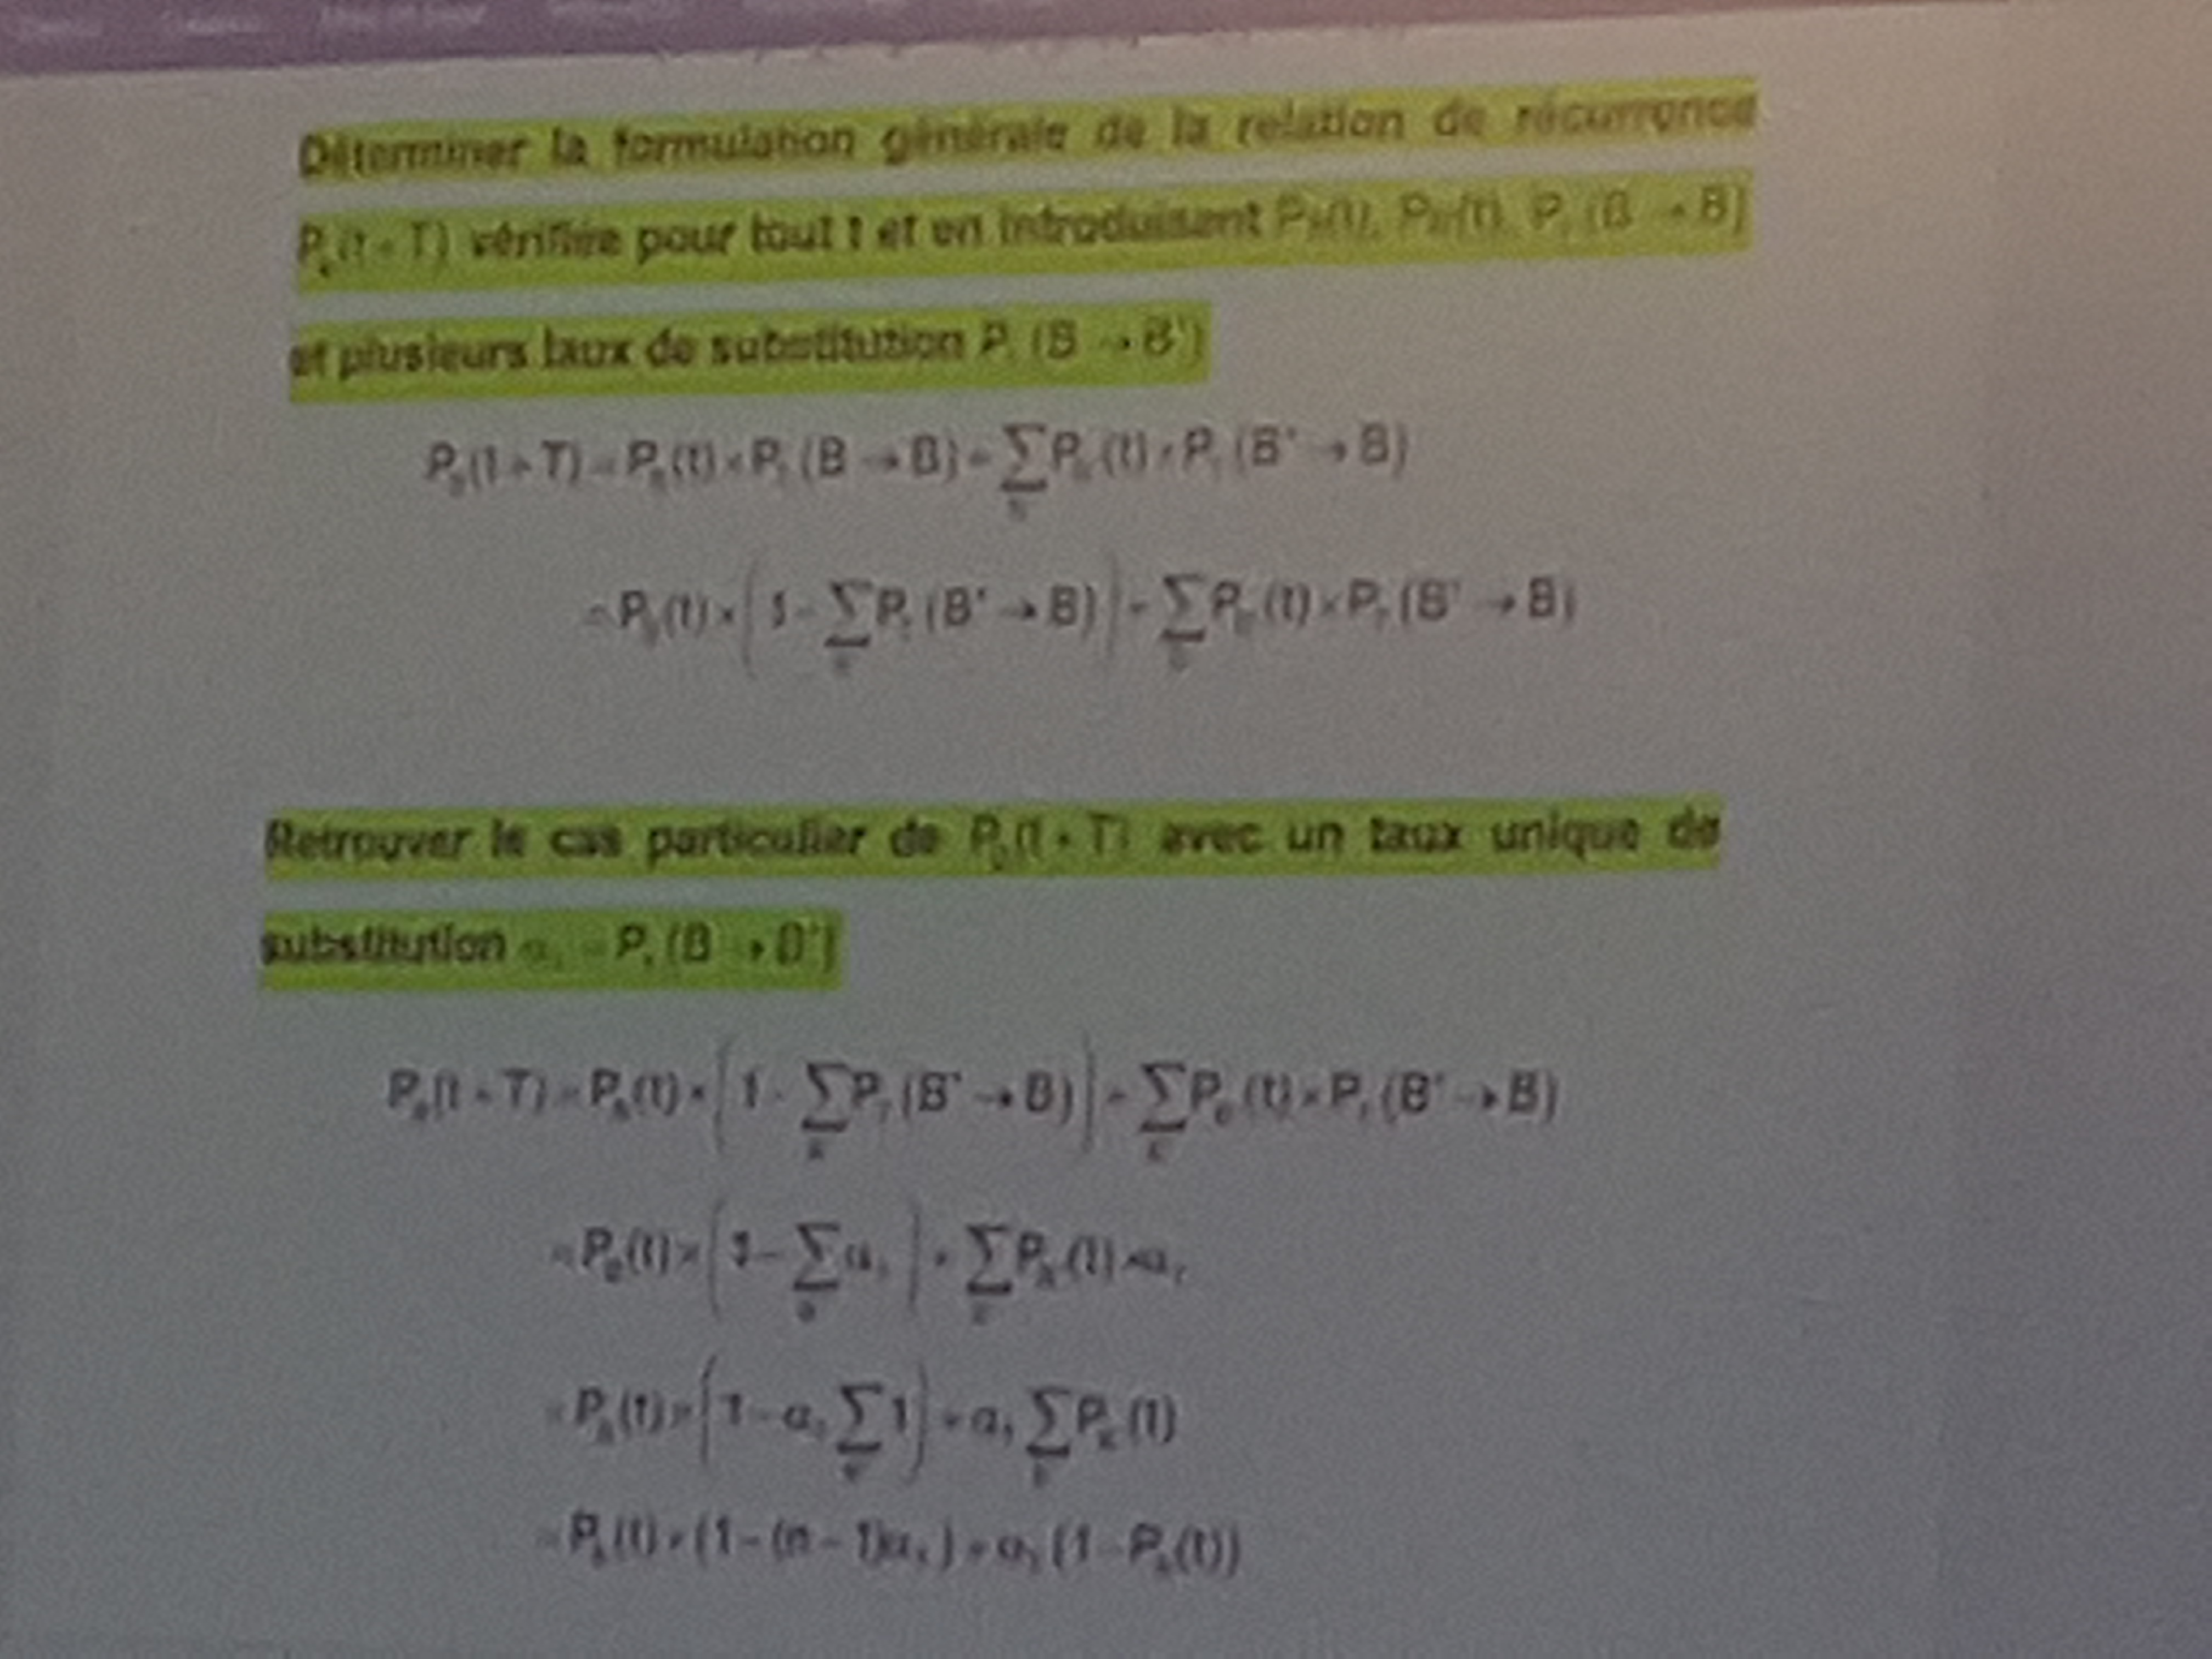
\includegraphics[width=0.99\textwidth]{img/cQuoiCetteMerde.jpg}
		\caption{Bonne chance pour lire}
	\end{figure}
	
%	Déduire $P_{B}(t + T) - P_{B}(t)$ pour un taux unique $\alpha_{T} = P_{T}(B \to B^{\prime})$ de substitution
%	$$P_{B}(t + T) - P_{B}(t) = -(n - 1)\alpha_{T}P_{B}(t) + \alpha_{T}(1 - P_{B}(t))$$
	
	Une formule au pif par le prof :\\
	
	\begin{align*}
		P^{\prime}_{B}(t) &= \lim\limits_{T \to 0}\left(\frac{P_{B}(t + T) - P_{B}(t)}{T}\right)\\
		&= \lim\limits_{T \to 0}\left(\frac{\alpha_{T}(1 - P_{B}(t)) - (n - 1)\alpha_{T}P_{B}(t)}{T}\right)\\
		&= (1 - P_{B}(t)) \lim\limits_{T \to 0}\left(\frac{\alpha_{T}}{T}\right) - (n - 1) P_{B}(t)\lim\limits_{T \to 0}\left(\frac{\alpha_{T}}{T}\right)\\
	\end{align*}
	Merci d'avoir effacé monsieur Michel <3\\
	
	\subsection{Déterminer l'approximation enter $\alpha_{T}$ et $\alpha$ quand $T \to 0$}
	$$\alpha_{T} \underset{T \to 0}{=} \alpha T$$
	
	\subsection{Simplifier $P_{B}^{\prime}(t)$}
	\begin{align*}
		P_{B}^{\prime}(t) &= (1 - P_{B}(t))\alpha - (n - 1)\alpha P_{B}(t)\\
		&= \alpha - \alpha P_{B}(t) - (n - 1)\alpha P_{B}(t)\\
		&= \alpha - n\alpha P_{B}(t)
	\end{align*}
	
	\begin{center}
		\begin{tabular}{|c|c|c|c|c|}
			\hline 
			& $A_{1}$ & --- & --- & $A_{n}$ \\ 
			\hline 
			$A_{1}$ & $1 - (n - )\alpha$ & $\alpha$ & $\alpha$ & $\alpha$ \\ 
			\hline 
			| & $\alpha$ & $1 - (n - )\alpha$ & $\alpha$ & $\alpha$ \\ 
			\hline 
			| & $\alpha$ & $\alpha$ & $1 - (n - )\alpha$ & $\alpha$ \\ 
			\hline 
			$A_{n}$ & $\alpha$ & $\alpha$ & $\alpha$ & $1 - (n - )\alpha$ \\ 
			\hline 
		\end{tabular} 
	\end{center}
\end{document}